\documentclass[11pt]{article}

\usepackage[margin=1in]{geometry}
\usepackage{amsmath,amssymb,amsthm}
\usepackage{enumitem}
\usepackage{hyperref}
\usepackage{tikz}
\usetikzlibrary{arrows.meta,positioning,shapes.geometric}

\title{Logic Verification and Dependency Map}
\author{(Generated summary from prior analysis)}
\date{\today}

\begin{document}
\maketitle

\begin{abstract}
This document audits the mathematical logic of the compiled writeup (``combined.tex'') at the level of
(i) internal correctness of the steps as written, (ii) the dependency structure between sections,
and (iii) identification of external inputs or unproven assumptions.
It also provides a flowchart describing how the sections and assumed results connect to reach the overall conclusion
(ground state existence/simplicity/positivity and symmetry).
\end{abstract}

\tableofcontents

\section{Scope of this audit}
This audit checks the \emph{logical} correctness of the argument structure:
\begin{itemize}[leftmargin=2em]
\item whether stated implications follow from the definitions and previously established lemmas,
\item whether the assembly of the operator-theoretic conclusions follows from the hypotheses listed,
\item and which steps rely on results treated as external inputs (rather than proved in-line).
\end{itemize}
It does \emph{not} independently re-derive the explicit formula identities for local terms (these are treated as inputs),
nor does it re-prove standard functional-analytic theorems unless the document explicitly does so.

\section{Correctness audit by module}

\subsection{Setup on $\mathbb R_+^\times$: convolution, involution, and correlation}
\paragraph{What is done.}
The document defines convolution/involution on $\mathbb R_+^\times$ (with multiplicative Haar measure),
introduces a unitary dilation representation $U_a$ on $L^2(\mathbb R_+^\times)$,
and specializes to functions of the form $f=g*g^*$.

\paragraph{Logic check.}
The key identities used are standard and consistent:
\begin{itemize}[leftmargin=2em]
\item $f(a)=\langle g, U_a g\rangle$ for $f=g*g^*$.
\item $f(a^{-1})=\overline{f(a)}$ for $f=g*g^*$.
\item The polarization identity for a unitary operator $U$:
\[
2\Re\langle \phi,U\phi\rangle \;=\; 2\|\phi\|^2-\|\phi-U\phi\|^2,
\]
which is repeatedly used to convert correlation terms into nonnegative difference energies.
\end{itemize}

\subsection{Local terms and truncation/disjoint-support facts}
\paragraph{What is done.}
The writeup introduces local distributions/terms $W_p(\cdot)$ and $W_{\mathbb R}(\cdot)$ as explicit formulas
and then proves truncation statements using support considerations (e.g.\ if $g$ is supported in an interval
then $\langle g,U_a g\rangle=0$ for sufficiently large $a$).

\paragraph{Logic check.}
The disjoint-support criterion is correct: if the dilation moves the support disjointly, the correlation vanishes.
This yields finiteness/truncation of several sums that appear later (notably the $p$-adic contributions).

\paragraph{Caveat (regularity/domain).}
The Archimedean integral formula defining $W_{\mathbb R}(f)$ can require regularity of $f$ for convergence near $x=1$.
Later, the operator-theoretic energy form is defined directly via translation differences, which is robust;
however, interpreting that form as \emph{equal} to a classical $W_{\mathbb R}(f)$ integral is only as rigorous
as the function class for which the explicit $W_{\mathbb R}$ formula is valid.

\subsection{Energy decomposition: prime and Archimedean pieces}
\paragraph{What is done.}
The document rewrites $-W_p(f)$ and $-W_{\mathbb R}(f)$ as sums/integrals of squared translation differences
plus a constant multiple of $\|g\|^2$, using:
\begin{itemize}[leftmargin=2em]
\item the unitary polarization identity,
\item truncation/disjoint-support,
\item and the logarithmic coordinate change $x=e^t$ that turns multiplicative dilations into additive translations.
\end{itemize}

\paragraph{Logic check.}
Both decompositions are logically correct:
\begin{itemize}[leftmargin=2em]
\item The $p$-term becomes a \emph{finite} weighted sum of $\|\widetilde G - S_{m\log p}\widetilde G\|^2$
(because only finitely many $m$ appear by truncation), plus a constant term.
\item The Archimedean term becomes an integral $\int w(t)\|\widetilde G - S_t\widetilde G\|^2\,dt$ plus a constant term,
and the tail $t>2L$ collapses to a constant multiple of $\|G\|^2$ by disjoint support.
\end{itemize}

\subsection{Definition of the difference-energy form and Markov property}
\paragraph{What is done.}
An energy form $\mathcal E_\lambda$ is defined on $L^2(I)$ (for an interval $I$) as a combination of:
\begin{itemize}[leftmargin=2em]
\item weighted sums of discrete translation differences, and
\item a weighted integral of continuous translation differences.
\end{itemize}
The Markov property is proved: normal contractions $\Phi$ satisfy $\mathcal E_\lambda(\Phi(\phi))\le \mathcal E_\lambda(\phi)$.

\paragraph{Logic check.}
The form is nonnegative by construction and the Markov (normal contraction) argument is correct:
it follows from the pointwise inequality $|\Phi(a)-\Phi(b)|\le |a-b|$ and the extension-by-zero compatibility when $\Phi(0)=0$.

\subsection{Zero indicator energy $\Rightarrow$ trivial sets}
\paragraph{What is done.}
A key lemma shows: if $B\subseteq I$ is measurable and $\mathcal E_\lambda(\mathbf 1_B)=0$,
then $B$ is null or conull in $I$.

\paragraph{Logic check.}
The chain of implications is correct:
\begin{itemize}[leftmargin=2em]
\item $\mathcal E_\lambda(\mathbf 1_B)=0$ forces $\mathbf 1_B$ to be translation-invariant
(for the family of translations appearing in the form) almost everywhere.
\item A continuity-in-translation step upgrades ``almost every translation'' to all translations in a neighborhood.
\item A standard mollification/translation-invariance argument then forces $\mathbf 1_B$ to be (a.e.) constant on $I$,
hence $B$ is null or conull.
\end{itemize}

\subsection{Operator realization and compact resolvent}
\paragraph{What is done.}
The energy form is realized as a closed, densely-defined form, hence induces a nonnegative selfadjoint operator $A_\lambda$.
A Fourier multiplier representation is used (for the ambient form on $\mathbb R$),
yielding a coercive control function $\psi_\lambda(\xi)$ with growth $\gtrsim \log|\xi|$ for large $|\xi|$.
Compactness of the embedding of the form domain into $L^2(I)$ is established (via translation control and Kolmogorov--Riesz),
implying that the resolvent is compact.

\paragraph{Logic check.}
This module is logically consistent:
\begin{itemize}[leftmargin=2em]
\item Closed form $\Rightarrow$ selfadjoint operator: correct (standard representation theorem).
\item Fourier representation and the multiplier formula for the translation-difference form: correct.
\item The lower bound $\psi_\lambda(\xi)\gtrsim \log|\xi|$ is consistent with the stated weight estimates
and is used in the correct direction (to force compactness via translation control).
\item The use of Kolmogorov--Riesz for compactness in $L^2$ is appropriate:
uniform translation control and tightness yield precompactness.
\item Compact resolvent follows from compact embedding and the resolvent-bounds-in-form-norm estimate.
\end{itemize}

\subsection{Irreducibility and Perron--Frobenius consequences}
\paragraph{What is done.}
The document uses standard Dirichlet form theory to pass from the ``indicator energy'' criterion
to irreducibility of the associated semigroup. Then it invokes a theorem of the form:
\begin{center}
positive $+$ irreducible $+$ holomorphic semigroup $\Rightarrow$ positivity improving,
\end{center}
and combines this with compact resolvent to conclude:
the principal eigenvalue is simple and has a strictly positive eigenfunction (ground state).

\paragraph{Logic check.}
The assembly is correct \emph{conditional on the cited/assumed semigroup theorems}.
The sequence:
\[
\text{Markov form} \Rightarrow \text{positive semigroup}
\Rightarrow (\text{indicator criterion}) \Rightarrow \text{irreducible}
\Rightarrow \text{positivity improving}
\Rightarrow \text{simple positive ground state (with compact resolvent)}
\]
is the standard Perron--Frobenius/Krein--Rutman/Jentzsch strategy for symmetric (or sectorial) Dirichlet forms.

\subsection{Reflection symmetry and even ground state}
\paragraph{What is done.}
The form is shown invariant under reflection on $I$ (e.g.\ $t\mapsto -t$ in logarithmic coordinates),
hence the operator commutes with reflection. Simplicity of the ground state forces it to be an eigenfunction of the symmetry,
and positivity selects the even (not odd) choice.

\paragraph{Logic check.}
This is correct: invariance of the form implies commutation at the operator level,
and a one-dimensional eigenspace is stable under commuting symmetries, hence yields an even ground state.

\section{External inputs and unproven assumptions}
The following items are \emph{not} proved from scratch inside the document and are treated as inputs
(standard or cited):

\begin{enumerate}[leftmargin=2.2em]
\item \textbf{Explicit local distribution formulas} for $W_p(f)$ and $W_{\mathbb R}(f)$ (explicit-formula local terms),
and the assumption that the chosen $f=g*g^*$ lies in the function class for which these formulas hold.
\item \textbf{Closed form $\Rightarrow$ selfadjoint operator} (representation theorem for closed quadratic forms; e.g.\ Kato/Friedrichs).
\item \textbf{Kolmogorov--Riesz compactness criterion} in $L^2(\mathbb R)$ (used to deduce compact embedding from translation control).
\item \textbf{Dirichlet form irreducibility equivalences:}
that the ``only trivial invariant sets'' criterion (often phrased via indicator functions)
is equivalent to semigroup irreducibility for the Markovian form.
\item \textbf{Positivity improving theorem:}
positive $+$ irreducible $+$ holomorphic semigroup $\Rightarrow$ positivity improving
(in the sense that nonzero $f\ge 0$ is mapped to a strictly positive function for $t>0$).
\item \textbf{Principal eigenvalue structure:}
positivity improving $+$ compact resolvent $\Rightarrow$ the lowest eigenvalue is simple
and the associated eigenfunction is strictly positive (Krein--Rutman/Jentzsch-type conclusion).
\end{enumerate}

\section{Logical flow summary (high level)}
The core argument proceeds in the following stages:

\begin{enumerate}[leftmargin=2.2em]
\item \textbf{Translate correlations into energies.}
Start with $f=g*g^*$ and identify the correlation $f(a)=\langle g,U_a g\rangle$.
Use the unitary polarization identity to write correlation terms as squared norms of translation differences.

\item \textbf{Use support to truncate.}
Support/disjointness shows $\langle g,U_a g\rangle=0$ beyond a cutoff, turning infinite sums into finite sums
and controlling tails.

\item \textbf{Logarithmic coordinate change.}
Convert multiplicative dilations into additive translations, allowing both prime and Archimedean local terms
to be expressed as translation-difference energies.

\item \textbf{Define the Dirichlet form $\mathcal E_\lambda$.}
Package the discrete (prime) and continuous (Archimedean) difference energies into a single Markovian quadratic form on $L^2(I)$.

\item \textbf{Establish irreducibility.}
Prove the indicator-energy lemma: $\mathcal E_\lambda(\mathbf 1_B)=0$ forces $B$ to be null or conull.
Invoke standard Dirichlet form theory to deduce semigroup irreducibility.

\item \textbf{Build the operator and spectral structure.}
Use closedness to produce the selfadjoint operator $A_\lambda$.
Prove compact resolvent by compact embedding of the form domain into $L^2(I)$ (via translation control/Kolmogorov--Riesz).

\item \textbf{Apply positivity improving $\Rightarrow$ Perron--Frobenius.}
Invoke the positivity improving theorem (from positivity + irreducibility + holomorphy),
then conclude simplicity and strict positivity of the ground state using compact resolvent.

\item \textbf{Exploit reflection symmetry.}
Show form invariance under reflection, hence $A_\lambda$ commutes with reflection,
and deduce the unique positive ground state can be chosen even.
\end{enumerate}

\section{Dependency flowchart}

\begin{center}
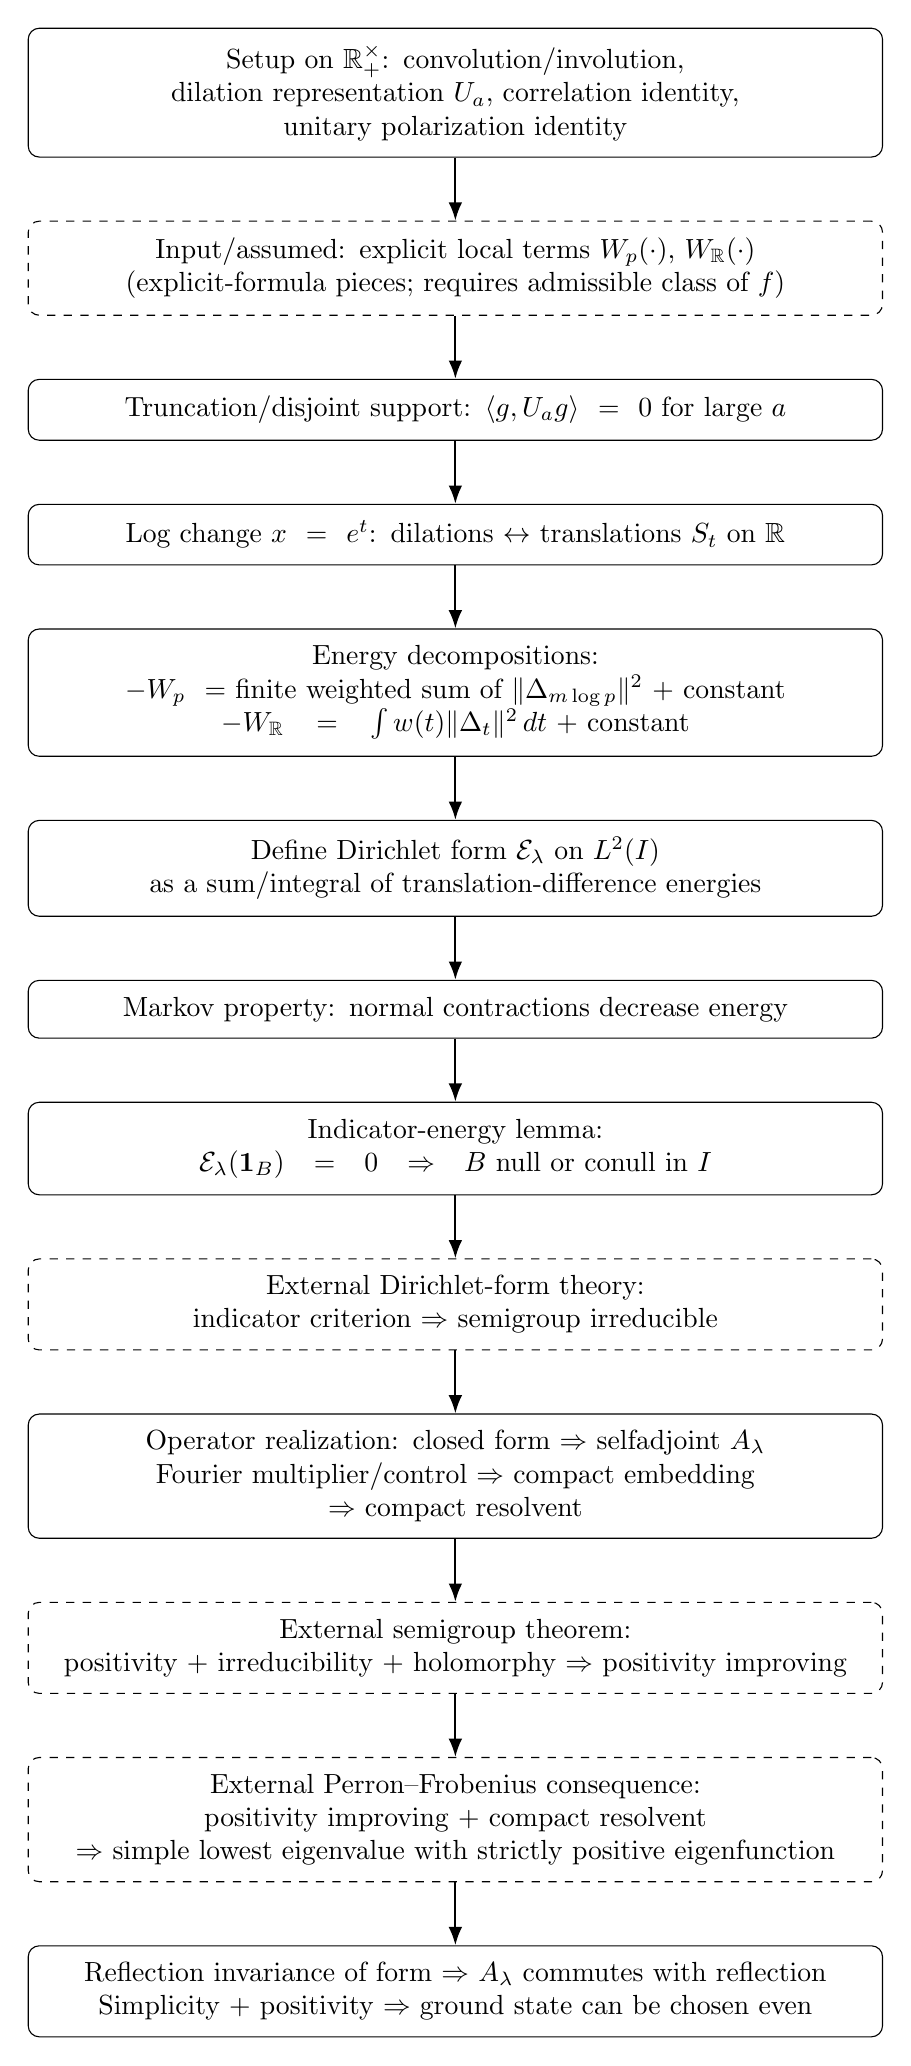
\begin{tikzpicture}[
  node distance=8mm and 10mm,
  box/.style={draw, rounded corners, align=center, inner sep=6pt, text width=0.86\linewidth},
  asum/.style={draw, dashed, rounded corners, align=center, inner sep=6pt, text width=0.86\linewidth},
  arr/.style={-Latex, thick}
]

\node[box] (setup) {Setup on $\mathbb R_+^\times$: convolution/involution,\\ dilation representation $U_a$, correlation identity,\\ unitary polarization identity};

\node[asum, below=of setup] (local) {Input/assumed: explicit local terms $W_p(\cdot)$, $W_{\mathbb R}(\cdot)$\\ (explicit-formula pieces; requires admissible class of $f$)};

\node[box, below=of local] (trunc) {Truncation/disjoint support: $\langle g,U_a g\rangle=0$ for large $a$};

\node[box, below=of trunc] (log) {Log change $x=e^t$: dilations $\leftrightarrow$ translations $S_t$ on $\mathbb R$};

\node[box, below=of log] (decomp) {Energy decompositions:\\ $-W_p =$ finite weighted sum of $\|\Delta_{m\log p}\|^2$ $+$ constant\\ $-W_{\mathbb R} = \int w(t)\|\Delta_t\|^2\,dt$ $+$ constant};

\node[box, below=of decomp] (form) {Define Dirichlet form $\mathcal E_\lambda$ on $L^2(I)$\\ as a sum/integral of translation-difference energies};

\node[box, below=of form] (markov) {Markov property: normal contractions decrease energy};

\node[box, below=of markov] (indicator) {Indicator-energy lemma:\\ $\mathcal E_\lambda(\mathbf 1_B)=0 \Rightarrow B$ null or conull in $I$};

\node[asum, below=of indicator] (irr) {External Dirichlet-form theory:\\ indicator criterion $\Rightarrow$ semigroup irreducible};

\node[box, below=of irr] (op) {Operator realization: closed form $\Rightarrow$ selfadjoint $A_\lambda$\\ Fourier multiplier/control $\Rightarrow$ compact embedding\\ $\Rightarrow$ compact resolvent};

\node[asum, below=of op] (posimp) {External semigroup theorem:\\ positivity $+$ irreducibility $+$ holomorphy $\Rightarrow$ positivity improving};

\node[asum, below=of posimp] (pf) {External Perron--Frobenius consequence:\\ positivity improving $+$ compact resolvent\\ $\Rightarrow$ simple lowest eigenvalue with strictly positive eigenfunction};

\node[box, below=of pf] (sym) {Reflection invariance of form $\Rightarrow$ $A_\lambda$ commutes with reflection\\ Simplicity $+$ positivity $\Rightarrow$ ground state can be chosen even};

\draw[arr] (setup) -- (local);
\draw[arr] (local) -- (trunc);
\draw[arr] (trunc) -- (log);
\draw[arr] (log) -- (decomp);
\draw[arr] (decomp) -- (form);
\draw[arr] (form) -- (markov);
\draw[arr] (markov) -- (indicator);
\draw[arr] (indicator) -- (irr);
\draw[arr] (irr) -- (op);
\draw[arr] (op) -- (posimp);
\draw[arr] (posimp) -- (pf);
\draw[arr] (pf) -- (sym);

\end{tikzpicture}
\end{center}

\section{Conclusion}
Internally, the argument is logically coherent:
the prime and Archimedean contributions are correctly rewritten as nonnegative translation-difference energies,
packaged into a Markovian closed form, and then pushed through standard Dirichlet form and positive-semigroup machinery
to obtain compact resolvent and a simple strictly positive ground state, with even symmetry by reflection invariance.

The principal nontrivial dependencies that remain external to the writeup are:
(i) the explicit-formula local term identities (and their domain of validity),
and (ii) standard operator/semigroup theorems (closed forms, irreducibility criteria, positivity improving, and Perron--Frobenius consequences).

\end{document}
